Throughout the development of Yarn, acceptance tests and specifications were
written prior to developing a feature. This provided a solid test coverage
which in turn allowed for some radical refactorings to improve the quality,
readability and performance of the system. By the end of development,
all 13 acceptance tests (Cucumber features) and 80 specifications (RSpec
specs) passed.  The final test coverage was 96.08\%, as depicted on
Figure~\ref{coverage}. 

\begin{figure}[htb]
  \centering
  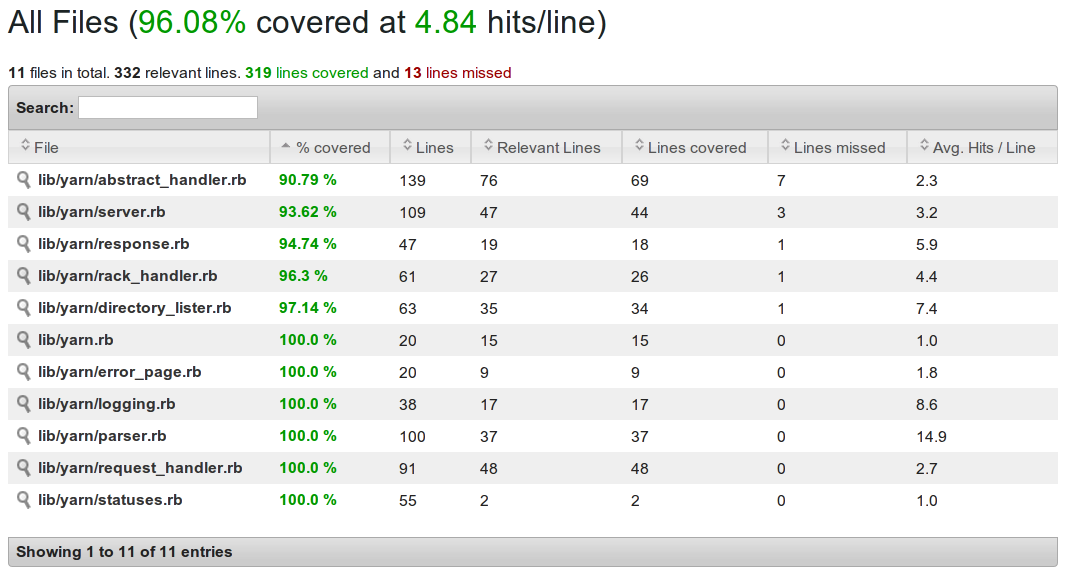
\includegraphics[width=0.9\textwidth]{img/coverage.png}
  \caption{Yarn test coverage screenshot.}
  \label{coverage}
\end{figure}

During the development, the test coverage was continously monitored to ensure
all parts of the system was exercised in the test suite. The test coverage
analysis is available on the CD in the \texttt{coverage} folder. The following
looks at how testing for concurrency was performed, and how the HTTP parser
was developed with BDD.

\section{Testing for Concurrency}
Some features were harder to test than others, and testing for concurrency was
especially tricky. The solution was to invoke two requests to a Ruby file, 
which invoked the \texttt{sleep} method for a given amount of time before
returning the response. Firing a request which slept for a second would block
other requests from being served during that second. But if the server could
handle concurrent requests, a fast request fired after the slow request,
should be able to get it's response prior to the slow request completing.
Listing~\ref{confea} shows the acceptance test for concurrent requests.

\bigskip
\begin{lstlisting}[label=confea,caption=Concurrency acceptance test
(features/concurrency.feature:7)]
Scenario: Perform two requests in parallel
  Given the server is running
  Given a client "A"
  And a client "B"
  When client "A" makes a "1" second request
  And client "B" makes a "0.1" second request
  Then client "B" receives a response before client "A"
\end{lstlisting}

Having this acceptance test proved especially valuable during the
reimplementation of the concurrency feature from using threads to using
processes.

\section{Testing the HTTP Parser}
The development of the HTTP parser was initiated by writing an acceptance test
as shown in Listing~\ref{parsacc}.

\bigskip
\begin{lstlisting}[label=parsacc,caption=HTTP parser acceptance test
(features/parser.feature:7).]
Scenario: Parse HTTP request
  Given a HTTP request "GET /index.html HTTP/1.1\r\nUser-Agent: cucumber\r\n"
  And a parser
  When I feed the request to the parser
  Then the result "method" should be "GET"
  And the result "uri" should include "path" with "/index.html"
  And the result "version" should be "HTTP/1.1"
  And the result "headers" should have "User-Agent" with "cucumber"
\end{lstlisting}

The acceptance test exercises the parser by supplying it with a HTTP request
string, and then expects the result to contain the values of the request.
Running the acceptance test revealed that the steps were not defined, and
implementing them was the next step. Listing~\ref{accstep} shows two of the step
definitions.

\bigskip
\begin{lstlisting}[label=accstep,caption=Parser step definitions excerpt
(features/step\_definitions/parser\_steps.rb:1).]
Given /^a parser$/ do
  @parser = Yarn::Parser.new
end

When /^I feed the request to the parser$/ do
  @result = @parser.run(@request)
end
\end{lstlisting}

With all the step definitions implemented, running the acceptance test again
revealed that the class \texttt{Yarn::Parser} did not exist. Creating the
class and running the test again revealed that the class did not have a method
named \texttt{run}. The development continued in this loop of first asserting
certain behavior from the code, discovering it did not behave as asserted, and
then implementing the expected behaviour.

Each element which should be parsed was added incrementally by first writing a
RSpec specification, and then adding the behaviour to the \texttt{Parser}
class. For instance, the expected behaviour of being able to parse query
parameters was written in a specification (Listing~\ref{queryspec}).

\bigskip
\begin{lstlisting}[label=queryspec,caption=Parser query parameter support specification (spec/yarn/parser\_spec.rb:54).]
it "parses query parameters in the URL" do
  result = Parser.new.run("GET /page?param1=1&param2=2 HTTP/1.1\n")
  result[:uri][:query].should == "param1=1&param2=2"
end
\end{lstlisting}

To begin with the parser is executed with a HTTP request. Then the result
\texttt{Hash} is inspected to see whether the values match. Running the above
specification would output an error message as the parser could not yet
handle the query parameter. The behaviour, Listing~\ref{quepars} was then
added to the \texttt{Parser} class.

\bigskip
\begin{lstlisting}[label=quepars,caption=URL query parameter support (lib/yarn/parser.rb:31).]
rule(:path) do 
  match['^\?'].repeat(1).as(:path) >> 
  str("?") >> 
  query.as(:query) | match['^\s'].repeat(1).as(:path)
end

rule(:query) do
  match['\S+'].repeat(1)
end
\end{lstlisting}

The behaviour added was lines 3,4 and lines 7 through 9. The path is checked
for the occurrence of a question mark, and if it is found the sequence of
characters until a whitespace character is parsed as the query string (line 8).

The implementation of all rules in the \texttt{Parser} class was developed
this way, totalling in 17 specs and one acceptance test for the
\texttt{Parser} class.


\section{Summary}
This chapter revealed how developing functionality through first describing
the expected behaviour in a test, worked out well and always made it clear
what the next step to completing a feature would be. It was also covered how
using a tool to monitor test coverage, ensured that all execution paths were
tested and thereby improved the value of the test suite.
In the next chapter the final version of Yarn is demonstrated and benchmarked.
